\chapter{Wstęp}

\section{Cel zajęć}
Celem niniejszej pracy była analiza oraz dobór parametrów systemu adaptacyjnego w zależności od występujących w systemie zakłóceń oraz transmitancji obiektu, którym sterowano. Przyjęty model przedstawiono na rysunku \ref{model_systemu}.

\begin{figure}[h!]
	\centering
	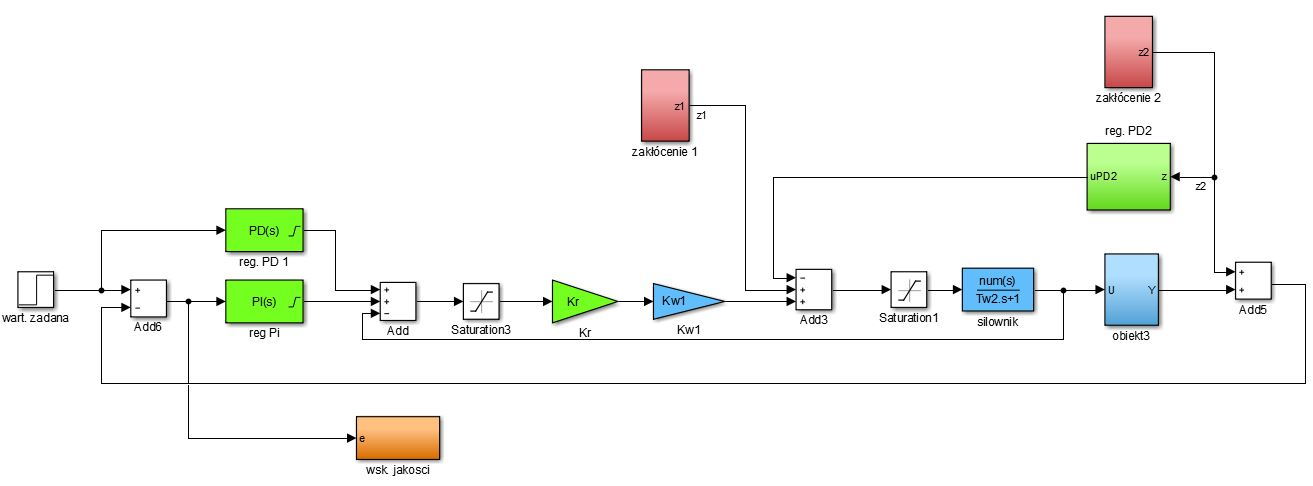
\includegraphics[scale = 0.6]{fig/model_systemu.png}
	\caption		
	{Model układu sterowania}
	\label{model_systemu}
\end{figure} 

\section{Model obiektu}

Obiektem sterowania był model Strejca, opisany  transmitancją:
\begin{equation}\label{key}
G(s) = \dfrac{K_0}{(T_0 \cdot s + 1)^n} \cdot e^{-\tau \cdot s} 
\end{equation}
Na potrzeby niniejszej pracy ograniczono się do obserwacji zachowania modeli rzędu pierwszego, drugiego oraz trzeciego.

\section{Regulatory}
Poszczególne regulatory znajdujące się na schemacie \ref{model_systemu} opisano następującymi wzorami: 
\begin{equation}\label{reg1}
PD_1 = \alpha_1+\beta_1 \cdot s
\end{equation}
\begin{equation}\label{reg2}
PD_2 = \alpha_2+\beta_2 \cdot s
\end{equation}\\
\begin{equation}\label{reg3}
PI = \gamma + \dfrac{\delta}{s}
\end{equation}
Element wykonawczy jest opisany za pomocą zależności:
\begin{equation}\label{actuator}
\dfrac{K_{w2}}{T_w s+T}
\end{equation}

Wartości parametrów $K_{w1}$, $K_{w2}$, $T_w$, $K_0$ potraktowano jako zadane. Przyjęto, iż testy zostaną przeprowadzone dla wartości zadanej $r$ dla pięciu różnych poziomów zmieniających się w zakresie $5-70^{\circ} C$. Zakłóceniem $z_1$ był niemierzalny skok $1(t)$, natomiast $z_2$ było mierzalnym skokiem $1(t)$.

W ramach projektu należało przeprowadzić optymalizację poszczególnych parametrów podanych powyżej regulatorów, tj. $\alpha_1$, $\beta_1$, $\alpha_2$, $\beta_2$, $\gamma$, $\delta$. Wskaźnikiem jakości, na mocy którego optymalizowano działanie całego układu, była całka z modułu uchybu:
\begin{equation}\label{wsk_jak}
J = \int |e(t)| dt
\end{equation}
gdzie: \\
$e(t) = r(t) - y(t)$ - uchyb regulacji.\\ 

 Ponadto przyjęto, iż oczekiwanym efektem optymalizacji będzie takie zachowanie układu, by bez względu na wartości zakłóceń $z_1$ i $z_2$, efekt stabilizacji był jak najlepszy.

